\chapter{Reconhecimento de Expressões Faciais}

\section{Introdução}
Segundo \citeonline{FernandoGil} "a expressão facial é uma forma de comunicação não-verbal que permite a partilha de
sentimentos e emoções, numa linguagem subentendida entre seres humanos". Desde o início das pesquisas na computação busca-se cada vez mais dotar o computador de um comprtamento inteligente. Sequindo esse caminho, o reconhecimento facial surgiu,  para trazer soluções no campo da Interface Home- Computador, como um desafio esperado, porém desafiador. Principalmente no reconheciemnto de expressões faciais, já que se trata de um julgamento ambíguo até mesmo para os seres humanos, pois a mesma expressão pode variar de indivíduo para indivíduo \cite{FernandoGil} \cite{Elizabeth}.

\section{Fasesdo Reconhecimeto}
O reconhecimento facial se divide em três etapas básicas \cite{Elizabeth}:
\begin{itemize}
\item Detectar a face na cena: Inicialmente é apresentada uma imagem contendo a face que deve ser rceonhecida. Nesta primeira etapa, deve ser realizada a detecção da zona da face, e devem ser extraídos os outros artefatos que não compõem o rosto \cite{FernandoGil}.
Na figura abaixo é ilustrado o resultado final desta primeira etapa.
\begin{center}
	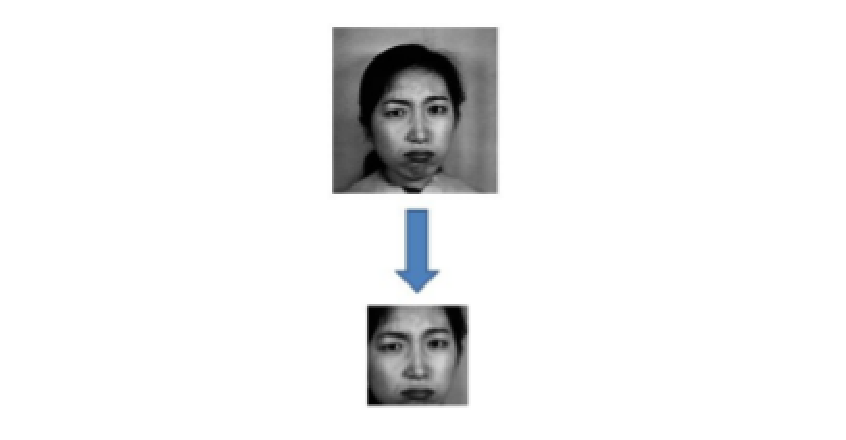
\includegraphics[scale=1.00]{graficos/rosto}
	\captionof{figure}{Detecção da face}
	\cite{Elizabeth}
\end{center}
\item Extrair as principais características: Nesta etapa são extraídas as características que são relevantes à classificação da expressão. Normalmente é dada maior ênfase as sobrancelhas, nariz, olhos e boca.
A figura abaixo mostra a seleção de pontos mais relevantes para a classificação da expressão
\begin{center}
	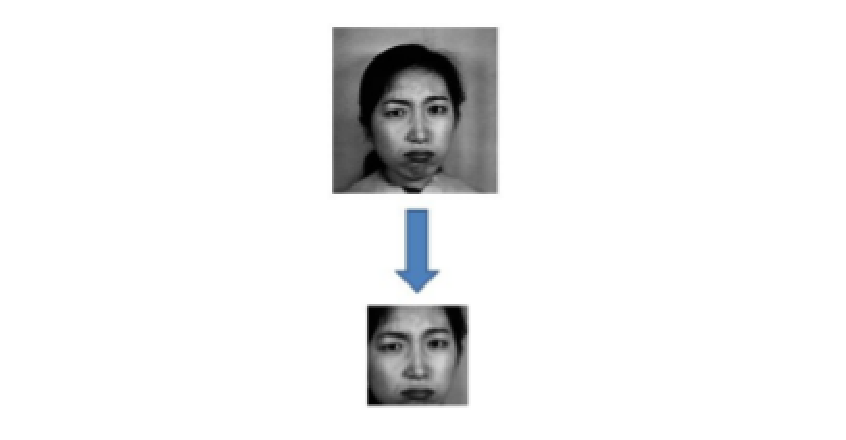
\includegraphics[scale=1.00]{graficos/rosto}
	\captionof{figure}{Pontos mais relevantes na face}
	\cite{Guo}
\end{center}
\item Classificar a imagem em uma detreminada expressão: Nesta etapa ocorre de fato a classificação da expressão. Para realizar esta classificação exitem diversos métodos, dos mais simples aos mais complexos.
\end{itemize} 

\section{Métodos de Classificação}
Em \citeonline{FernandoGil} é descrito um método onde é utlizada uma base de dados com imagens de diferentes indivíduos relativas às expressões. A face a ser classificada é associada a face mais semelhante dentre as existentes na base dados, e após isso a expressão é classificada. Este método parte do princípio que pessoas com fisionomias semelhantes possuem uma maneira similar de apesentar a mesma expressão. Através de uma estrtura denominada General Face Knowledge são criados grafos sobre as imagens, através de pontos-chave da face. Quando o grafo do rosto, a ter sua expressão reconhecida, é criado, este é comparado aos grafos das imagens da base de dados, para que uma face semelhante seja enocntrada. Na figura abaixo é ilustrado uma grfao sobre uma face. Esta abordagem obteve uma taxa de sucesso de cerca de 89\%.
\begin{center}
	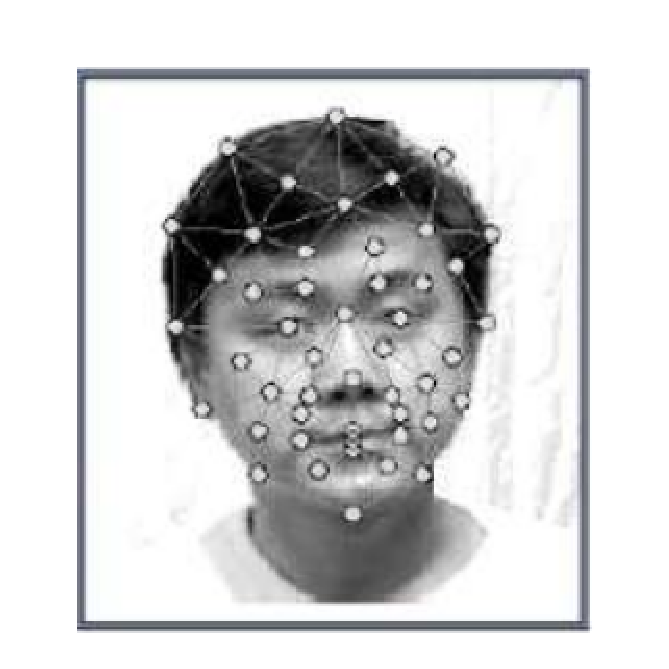
\includegraphics[scale=1.00]{graficos/metodo1_classi}
	\captionof{figure}{Exemplo de aplicação de General Face Knowledge ao rosto}
\end{center}

\citeonline{FernandoGil} apresenta ainda um outro método. Este método utiliza um framework denominado Active Appearance Models, nessa abordagem o objetivo é detectar a face idenpedente da luminosidade e posição. O  Active Appearance Models
possui um modelo estático que deve se ajustar a face que está sendo analisada através de alguns parâmetros e de forma iterativa.
\begin{center}
	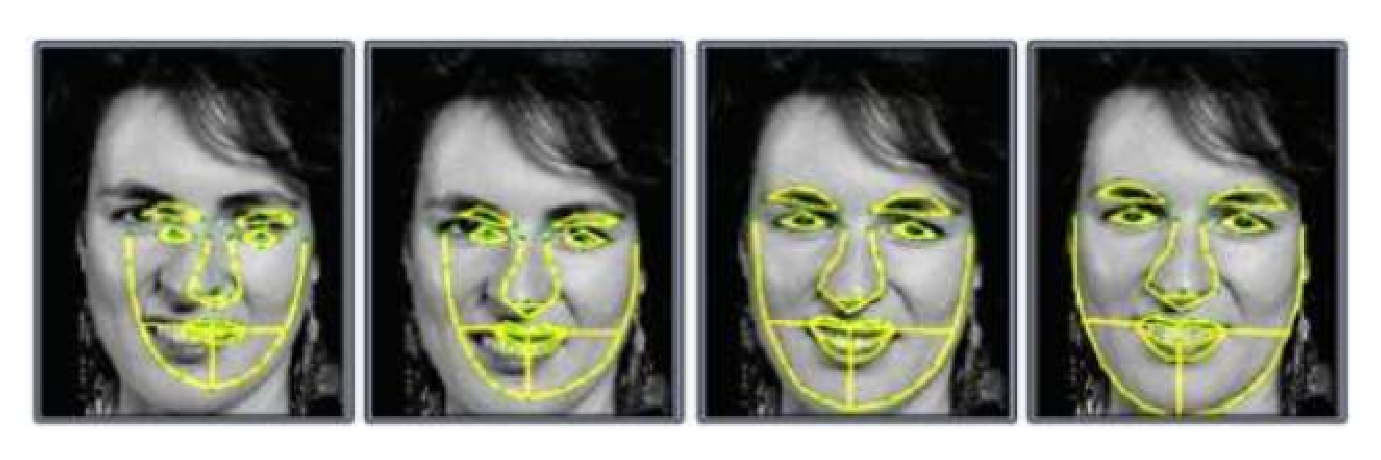
\includegraphics[scale=1.00]{graficos/metodo2_classi}
	\captionof{figure}{Ajuste do Active Appearence Models em três iterações a partir da posição inicial}
\end{center}

Em um outro trabalho também citado por \citeonline{FernandoGil} são definidas características-modelo, que são comparadas às características da face neutra, ou seja, sem expressar emoção, do indivíduo que está sendo analisao. Após essa etapa, é analisada a deformação, em relação ao modelo, quando o indivíduo expressa alguma emoção. A partir da deformação é realizada a classificação da expressão. A taxa de sucesso é de 92\% para a metade superior da face e de
86\% para a metade inferior. Na imagem a seguir é ilustrado o ajustamento das características modelo ao olho.
\begin{center}
	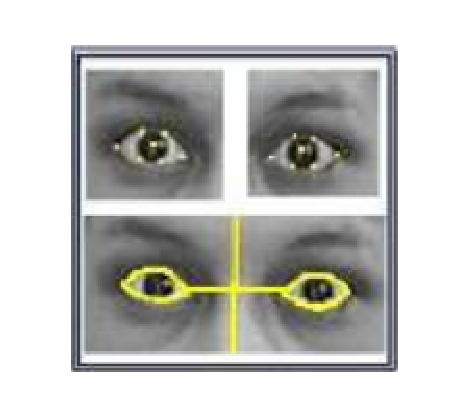
\includegraphics[scale=1.00]{graficos/metodo3_classi}
	\captionof{figure}{ Ajustamento ao olho: características-modelo}
\end{center}
\section{A Programação Linear e o Reconhecimento de Expressões Faciais}
